\documentclass[10pt,twocolumn,letterpaper]{article}

\usepackage{cvpr}
\usepackage{times}
\usepackage{epsfig}
\usepackage{graphicx}
\usepackage{amsmath}
\usepackage{amssymb}
\usepackage{subcaption}

% Include other packages here, before hyperref.

% If you comment hyperref and then uncomment it, you should delete
% egpaper.aux before re-running latex.  (Or just hit 'q' on the first latex
% run, let it finish, and you should be clear).
\usepackage[breaklinks=true,bookmarks=false]{hyperref}

\cvprfinalcopy % *** Uncomment this line for the final submission

\def\cvprPaperID{****} % *** Enter the CVPR Paper ID here
\def\httilde{\mbox{\tt\raisebox{-.5ex}{\symbol{126}}}}

% Pages are numbered in submission mode, and unnumbered in camera-ready
%\ifcvprfinal\pagestyle{empty}\fi
\setcounter{page}{1}
\begin{document}

%%%%%%%%% TITLE
\title{Generating Audio for Muted Piano-Playing Video Using Deep Learning \newline \newline \textit{Project Milestone}}


\author{XIA Junzhe\\
\tt\small 20493411\\
{\tt\small jxiaaf@connect.ust.hk}
\and
YANG Baichen\\
\tt\small 20493198\\
{\tt\small byangak@connect.ust.hk}
\and
HUANG Zeyu\\
\tt\small 20493631\\
{\tt\small zhuangbi@connect.ust.hk}
}


\maketitle
%\thispagestyle{empty}

%%%%%%%%% BODY TEXT
\section{Introduction}

It is noticed that human playing the piano effectively generates a series of well-patterned actions,
i.e. the position of hands and the keys and the depth of keys being pressed down.
The notes that the piano generates strongly obey to this visual pattern.
Hence, it becomes reasonable to recognize the visual patterns from piano-playing videos and reproduce the instrumental sounds using machine learning.

In this project, we aim to adapt some deep learning techniques related to object detection into this task and build a more robust model to detect what keys are being pressed in the video as well as the velocity of every single key press, which will enable us to retrieve the notes which are sounded. 
After the note sequence is obtained, we will use some software instrument to reproduce the piano sound and remix it with the original video. 
Apart from the basic task just mentioned, we also hope to make this model support real-time audio generating, which may require us using some faster network architectures like Faster R-CNN and cope with the synchronization between the detected notes and the audio to be generated.

% In this project, we aim to achieve hand gesture detection in piano playing and generate the correponding audio afterwards.
% It is also expected that we can thereby generate piano sound by our model without a real sound-producing piano, but only with a ``fake" one.

\section{Problem Statement}
In this section we will mainly discuss our problem statement, introducing our dataset sources, the evaluation patterns and expected results.

\subsection{Dataset Source}
\label{source}

To generate instrumental audio from piano-playing videos by recognizing hand gestures, we need a piano-video dataset where each frame must contain the whole keyboard, since it's almost impossible to determine the pitch of a note without a complete keyboard view.
Also, the required video dataset should be clear enough to demonstrate hand actions. And it's better for the dataset to expose the pitch information.

According to the above requirements, we find a suitable dataset, which is used in some related research \cite{Akbari}. It consists of several muted videos and their corresponding MIDI files, which exposes the pitch information.
However, there are still labelling and localization work to be done on the dataset to perform training on it. These tasks have already been accomplished and will be discussed in Section \ref{result}.

\subsection{Evaluation and Expected Result}
\label{evaluation}

Our eventual output will be a MIDI file containing a series of notes generated from the visual deep learning results. We expect the audio to correspond to the provided video. Specially, if the video is of playing a piece of musical work, the audio should sound natural and harmonic.

To evaluate the performance of our networks, we will compute each note's duration difference between the original file and our output. Summing the differences up, we will get a total time length of difference as a quantified evaluator of our network. Since each note has its pitch and duration quantified in the MIDI file, computing the difference is easily achievable.

Besides, we can set up a survey platform and invite people to judge whether the music we generate from playing musical work is natural.

If our network is well-trained, we expect the total difference to be small, and people to be likely to think our generated music is natural.

\section{Technical Approach}
\label{approach}

In this section, we will discuss the approaches we propose to achieve the objectives.

\subsection{Improving Keyboard Detection}

In the very beginning, we need to extract the boundary of the piano keyboard in the video. Instead of using the traditional CV method to extract coordinates of four corners of the keyboard which is utilized in previous work \cite{Akbari}, we will use CNN to perform this task. This is because the deep learning method has relatively better robustness and efficiency. Details will be discussed later in Section \ref{keyboardDetection}.

\subsection{Keyboard Separation Algorithm}

After the keyboard can be correctly recognized, we will use perspective transformation to normalize the keyboard in video frame into a preset rectangle structure. Then we will work on an algorithm to extract boundaries of each key, namely, further separate the keyboard into individual keys on this.

\subsection{Training Key Recognition Network}

When individual keys can be localized and normalized, it is feasible for us to perform deep learning on each key to determine their conditions (pressed or not pressed). The quality of the eventually generated music heavily depends on the performance of this network.

\subsection{Training Velocity Detection Network}

A music piece without emotional variation is rigid and undesired. To detect the velocity information of a key pressing event, we propose a recurrent network to analysis relative frames in order to derive an approximate velocity value of this pressing.

\subsection{Audio Generation}

Upon we can derive all notes information, we need to reconstruct them as a MIDI file. During this process, we may need to smooth out some noisy notes such as those with exceptionally short duration. Besides, it may be necessary to normalize the velocity information we retrieved to avoid unexpected dynamic change.

\section{Preliminary Results}
\label{result}

\subsection{Deep Learning Based Keyboard Detection}
\label{keyboardDetection}

Among all of the previous work that we have studied, no deep learning based method is used to localize the keyboard in video frame. Instead, all of them used traditional CV method such as Hough Line Transformation, brightness comparison to determine the coordinates of four corners of the piano keyboard (Fig.\ref{fig:1}). We have first partially reproduced this algorithm.

\begin{figure}[h!]
  \begin{subfigure}{0.23\textwidth}
    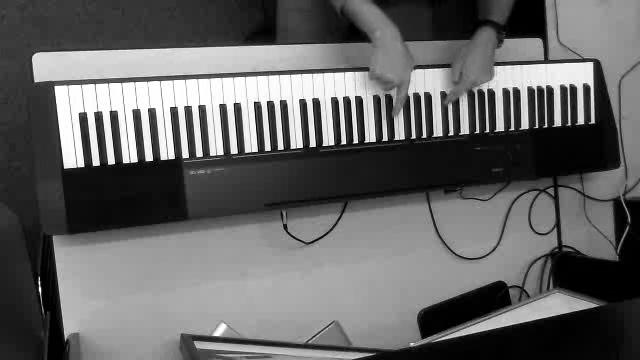
\includegraphics[width=\linewidth]{fig/1.jpg}
    \caption{Grayscaled Original Image} \label{fig:a}
  \end{subfigure}\hspace*{\fill}
  \begin{subfigure}{0.23\textwidth}
    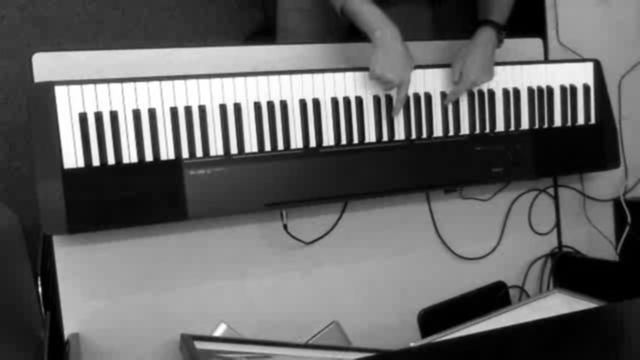
\includegraphics[width=\linewidth]{fig/3.jpg}
    \caption{Gaussian Blurred Image} \label{fig:b}
  \end{subfigure}
  
  \medskip
  \begin{subfigure}{0.23\textwidth}
    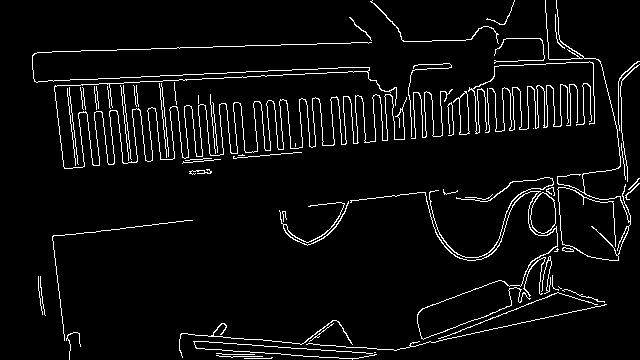
\includegraphics[width=\linewidth]{fig/4.jpg}
    \caption{Canny Edge Detection} \label{fig:c}
  \end{subfigure}\hspace*{\fill}
  \begin{subfigure}{0.23\textwidth}
    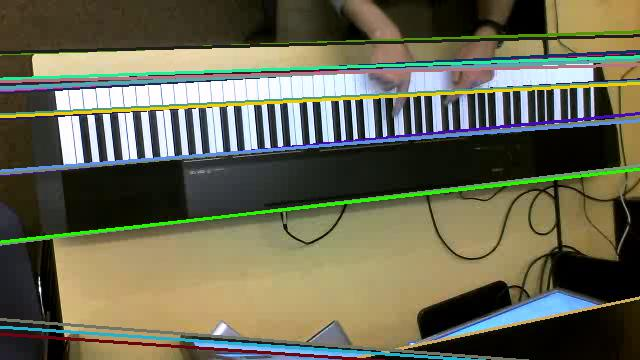
\includegraphics[width=\linewidth]{fig/5.jpg}
    \caption{Hough Line Transformation} \label{fig:d}
  \end{subfigure}
  
  \medskip
  \hspace{2.1cm}
  \begin{subfigure}{0.23\textwidth}
    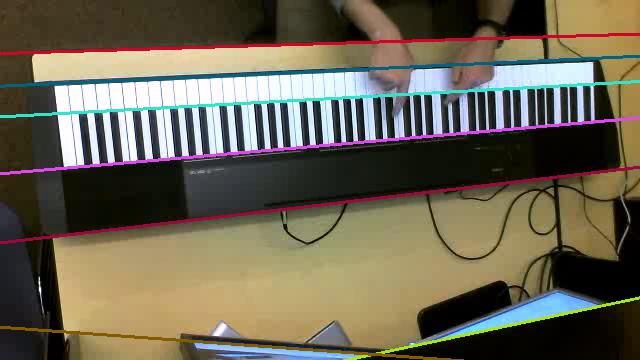
\includegraphics[width=\linewidth]{fig/6.jpg}
    \caption{Prune Repeated Lines} \label{fig:e}
  \end{subfigure}\hspace*{\fill}
  
  \caption{Pipeline of Finding Boundaries of Keyboard} \label{fig:1}
\end{figure}

After pruning repeated lines, some hard-coded method will be used to finally determine the positions of four corners. However, after applying this method to multiple images with different light conditions and hand positioning, we found the following drawbacks:

\begin{itemize}
  \item To achieve a satisfying performance, several hyperparameters in Hough Line Transformation and Canny Edge Detection needs to be adjusted dramatically in different images.
  \item To accurately determine the corners' coordinates, it is required there is no hands posing above the keyboard. It is hard to guarantee since most of piano videos do not contain such a "empty" frame. In some cases, the camera angle will even change slightly, where the traditional method will fail.
\end{itemize}

Due to the weak robustness of the traditional CV method, we decided to use a convolutional neural network to localize coordinates of four courners of the keyboard. However, we do not have any existing dataset for this task. So we labelled a number of images (Fig. \ref{fig:2}) captured from different piano playing videos, which come from the dataset of a previous research project, as well as some videos on the Internet.

\begin{figure}[h!]
  \hspace{2.1cm}
  \begin{subfigure}{0.24\textwidth}
    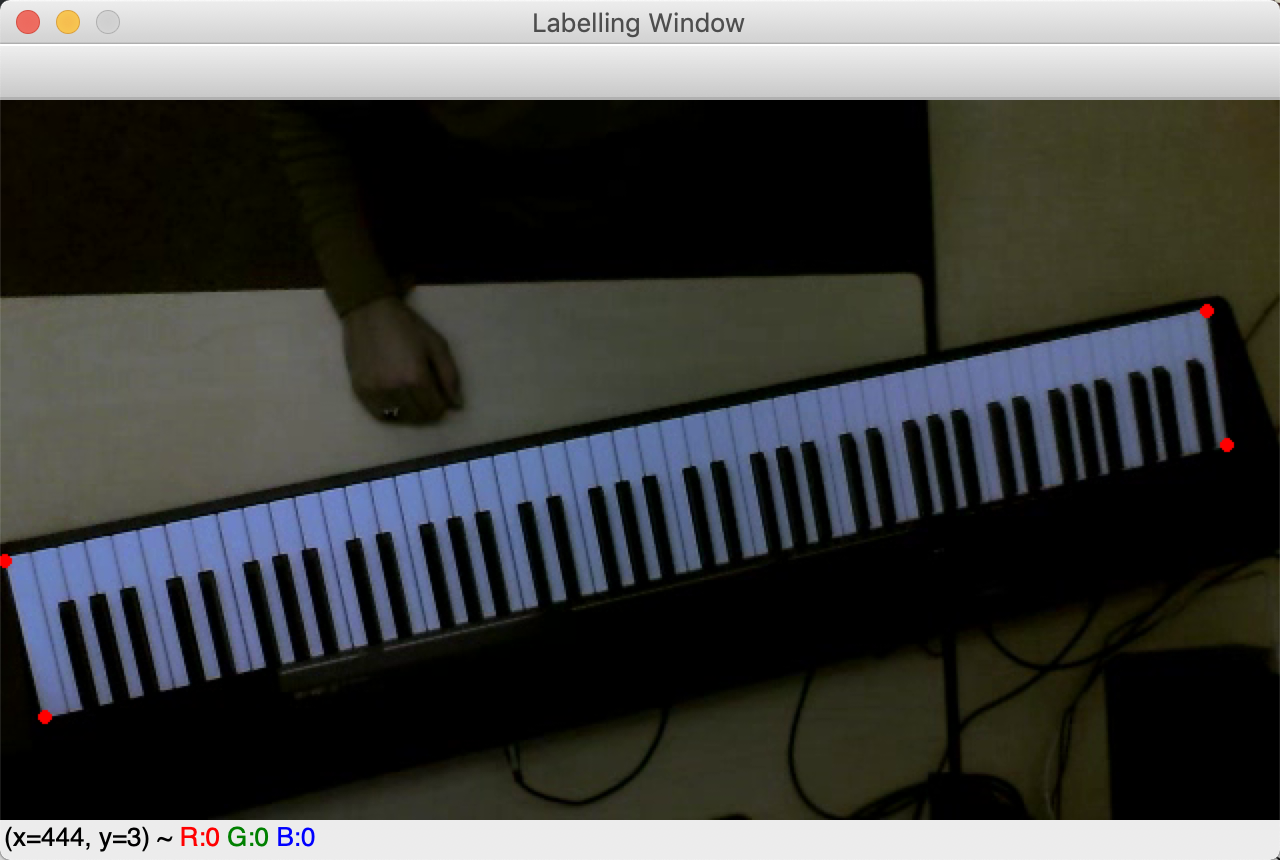
\includegraphics[width=\linewidth]{fig/7.png}
  \end{subfigure}
  \caption{Labelling Tool}
  \label{fig:2}
\end{figure}

To augment this dataset, we also consider artificially putting keyboard images onto some random backgrounds and perform some basic transformation such as flipping and stretching on images present.

In parallel with augmentation of the dataset, we have also started to evaluate the performance of several different CNNs on this task.

\subsection{Dataset Pre-process}


Currently we've conducted some pre-processing on the dataset and got the following preliminary results.

As mentioned in Section \ref{source}, the dataset we found only consists of several videos and corresponding MIDI files. 
So our very first task is to expose the pitch information from the MIDI files and store the mapping from each video frame to the sounded notes of that frame.

We fulfilled this task by first extracting all frames from the videos and the notes information from the MIDIs. We then construct and store the mapping as a \textit{numpy} array of size $(N, 128)$, where $N$ represents the number of frames and $128$ stands for the number of pitch possibilities in MIDI file format.
Each entry of the array has the value of either $1$ or $0$, where $1$ represents ``note\_on'' and $0$ stands for ``note\_off''. Through this data structure, we can easily form a correspondence between frames and notes. And in consistent with expectation, frames and notes are matched perfectly according to our testing result.

As for the keyboard localization network, we have already collected and labelled some videos from YouTube, as is mentioned above.

\section{Future Work}
In the future, there is plenty of work to be done.

\subsection{More Refining on the Dataset}

  
While we are labelling the data, we have found several shortcomings of the dataset:
\begin{itemize}
  \item The fake gestures are almost identical, which is moving the palms above the keyboard horizontally back and forth after finishing playing. This pattern may not be able to represent all kinds of visual interference.
  \item A large portion of the dataset is pressing the keys slowly from left to right one by one using only one finger. This playing pattern sheds less shadow and causes less interference than playing the piano in the real world.
  \item Several audio files are corrupted. Either they are empty or the midi messages have messed up timing information. Moreover, the leftmost key and the rightmost two keys are broken and not recorded into the MIDI file.
  \item Only one or two from the 14 players play meaningful pieces instead of random fiddling. We think more meaningful pieces should be included, since playing some common chords may generate some exclusive yet common and critical graphic information.
\end{itemize}

Given the shortcomings mentioned above, we believe that it is helpful to add our own dataset, where, beside avoiding these problems, we can also provide the following enhancements

\begin{itemize}
  \item The keyboard localization data.
  \item The ``strength'' information upon pressing a key.
\end{itemize}

We plan to record our own videos after the milestone, in parallel with the training process.

\subsection{Tuning the Networks}

To achieve our goals of keyboard localization, key detection and velocity detection, we will build and tune several separate networks. Details are covered in Section \ref{approach}.

\subsection{Conduct Evaluation on the Result}

As is described above in Section \ref{evaluation}, we will eventually build an evaluation system to evaluate the difference between our output and the original music file. We would like to minimize this difference during our experiments.

{\small
\bibliographystyle{ieee}
\bibliography{egbib}
}

\end{document}
